\subsection{Confounding-sensitivity analysis for JOBS II}

Using the same participants and baseline variables, we fit the reduced-form extension over $\rho\in[-0.8,0.8]$. The three-regression stack and its complete nuisance covariance provide a self-contained calculation of the sensitivity functionals and their uncertainty. Its finite-sample $\rho=0$ results complement the primary conditional-outcome estimates in Table~\ref{tab:application_effects} as a distinct reduced-form analysis.

\begin{table}[htbp]\centering\small\setlength{\tabcolsep}{4pt}
\caption{JOBS II reduced-form sensitivity analysis. Nominal intervals are pointwise working-model intervals. The zero-effect correlation is conditional on a nonzero mediator treatment effect.}
\label{tab:confounding-thresholds}
\begin{tabular}{llrrr}\toprule
Effect & Method & Effect at $\rho=0$ (95\% CI) & $\widehat\rho^\dagger$ (95\% CI) & $(\widehat\rho^\dagger)^2$\\\midrule
PNIE & OLS-RF & -0.012 [-0.032, 0.008] & -0.231 [-0.334, -0.122] & 0.053\\
TNIE & OLS-RF & -0.010 [-0.028, 0.007] & -0.213 [-0.292, -0.130] & 0.045\\
PNIE & DS-RF & -0.015 [-0.028, -0.002] & -0.244 [-0.345, -0.137] & 0.059\\
TNIE & DS-RF & -0.013 [-0.025, -0.002] & -0.222 [-0.300, -0.142] & 0.049\\
\bottomrule\end{tabular}\end{table}


We use the additional variance-decomposition interpretation of \citet{imai2010a}. Let $R_M^{2*}$ and $R_Y^{2*}$ denote the residual variance fractions explained by a hypothetical pretreatment confounder. The calibration is $\rho=s\sqrt{R_M^{2*}R_Y^{2*}}$, where $s\in\{-1,1\}$ specifies opposite or matching confounder-effect signs. Figure~\ref{fig:confounding-contours} shows both signs. The axes quantify residual-variance fractions and are distinct from the total-variance quantities $\widetilde R_M^2,\widetilde R_Y^2$. This working calibration translates specified latent variance contributions into sensitivity values; the one-dimensional PNIE/TNIE curves appear in Figure~S6.

\begin{figure}[htbp]
\centering
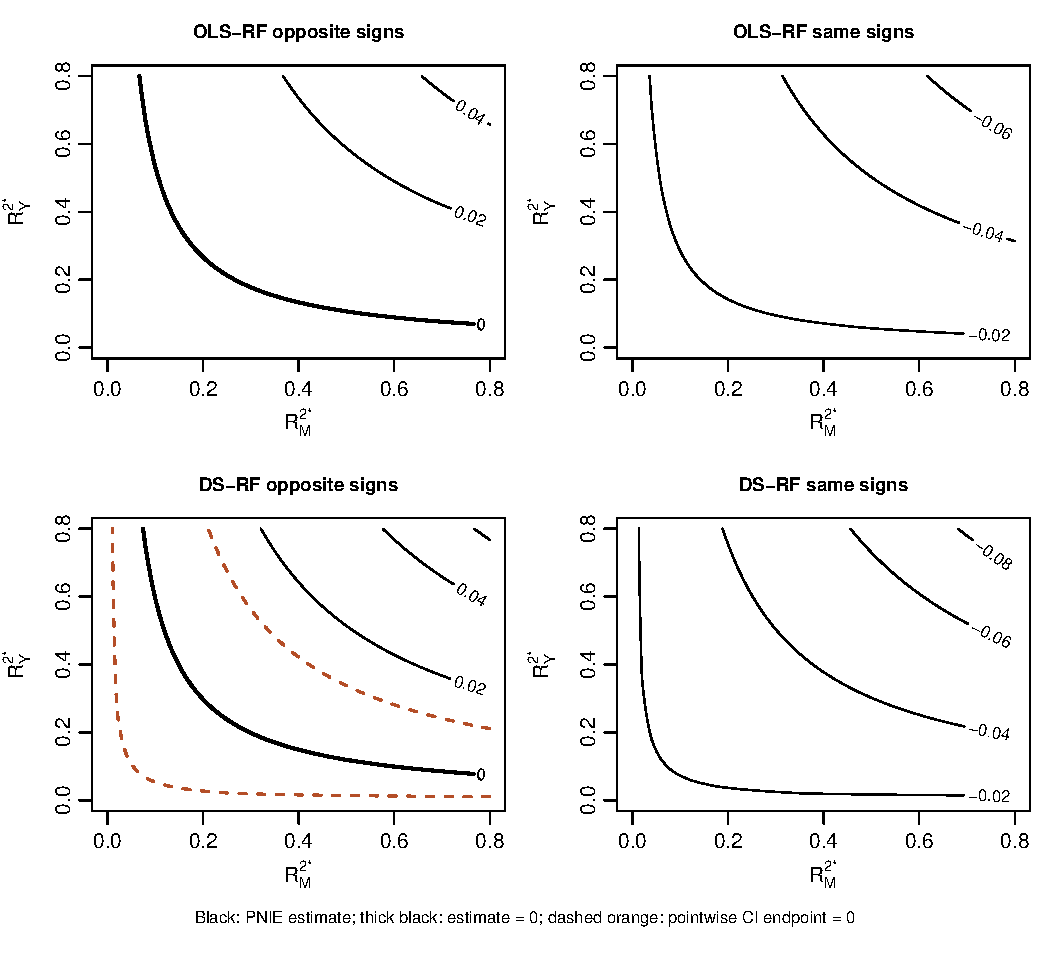
\includegraphics[width=0.92\textwidth]{figures/confounding_r2_contours.pdf}
\caption{JOBS II PNIE sensitivity contours from OLS-RF and DS-RF. Each black curve gives combinations of hypothetical residual-variance fractions yielding the labeled point estimate. The thick zero contour concerns the point estimate when crossed in the displayed grid; dashed orange curves mark a pointwise nominal interval endpoint equal to zero. Both confounding signs are shown. The contours are interpreted under the reduced-form working model and alongside the residual-variance diagnostics.}
\label{fig:confounding-contours}
\end{figure}

At $\rho=0$, OLS-RF gives PNIE $-0.0116$ with nominal interval $[-0.0316,0.0084]$, whereas DS-RF gives $-0.0149$ with $[-0.0284,-0.0015]$. The corresponding DS-RF TNIE is $-0.0132$ with $[-0.0246,-0.0018]$. The estimated correlations at which the point estimates cross zero are $-0.231$ for OLS-RF and $-0.244$ for DS-RF for PNIE, corresponding to residual-$R^2$ products of 0.053 and 0.059; TNIE gives $-0.213$ and $-0.222$. Thus opposite-sign confounder associations explaining roughly 5--6\% of the two residual variances in product provide a useful calibration for the estimated zero boundary. The close boundary estimates agree with their shared first-order residual-moment representation, while the shorter DS-RF intervals reflect the regression-coefficient contribution to curve estimation. Reduced-form variance diagnostics give reference $p$-values of 0.024 for the pooled mediator model and 0.009 and 0.006 for the two DS-RF outcome strata. The sensitivity curves are therefore interpreted as pointwise working-model summaries alongside the variance diagnostics and causal assumptions.

\FloatBarrier
